%experiment
SLM-Toolkit ist ein Werkzeug von Roni Rosenfeld,das angegebene Text bearbeit und folgende Ausgabe erzeugt\cite{int_slm_toolkit}:
\begin{itemize}
	\item word frequency lists and vocabularies
	\item word bigram and trigram counts
	\item vocabulary-specific word bigram and trigram counts
	\item bigram- and trigram-related statistics
	\item various Backoff bigram and trigram language models
	\item perplexity - Out-Of-Vocabulary (OOV) rate 
	\item bigram- and trigram-hit ratios
	\item distribution of Backoff cases 
	\item annotation of test data with language scores 
\end{itemize}

Das Software gibt beim Sprachmodell auch "`absolute"', "`good\_turing"' and "`witten\_bell- Discounting"' an.
F\"ur bestimmt Ziel muss man nicht alle Software ausf\"uhren. Abbildung (3.1) ist eine typische Anwendung, die Datenfluss und Operationfluss zeigt.
Ein Training-kurps ist am Anfang eingegeben und nach Modellierungsverfahren wird ein Sprachmodell ausgegeben


\begin{figure}[h]
	%\centering
	%\centering
	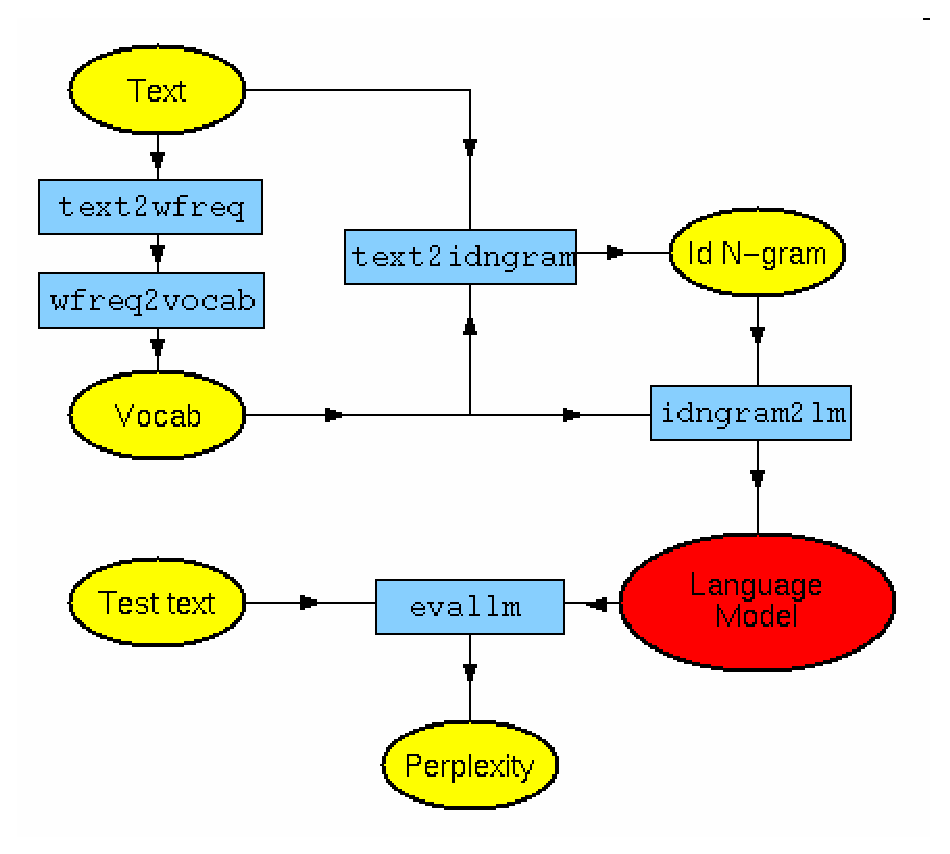
\includegraphics[width=0.5\textwidth]{bilder/toolkit.eps}
	 \caption{Flussdiagramm der typische Anwendung}
  \label{fig:figure_2}
\end{figure}

Bei Auswahl der Trainingkorpus und Testkorpus muss man sorgf\"altig entwerfen. \cite{book_speech} deutet uns einige Regele an, dass Trainingkorpra nicht zu spezifisch f\"ur die Aufgabe und auch nicht zu allgemein sein sollen.  

In unseren Experimenten verwenden wir die WSJ(Wall Street Journal) Sprachdatenbank, erhalten wir die Testergebniss von unterschiedlich Discounting und M-Gramm-Modell. In den Experimenten werden am Ende die Parameter \emph{backoff\_from\_unk\_inc} und \emph{backoff\_from\_unk\_exc} beim Entropieberechen eingesetzt.  
 Aber wir haben auch eine Problem gefunden, dass bei Absolute-Discounting man nur NAN bekommen kann, wenn man mit komplette wsj-Databasis arbeiten, weil die Vokabulargr\"o\ss e von 65535 beschr\"anket werden. In Tabelle 3.1 gebe ich nur verringerte Trainingbasis (Trainingdaten aus Verzeichnis 88 und Testdaten "`pp\_et\_05.nvp"'). Die Testdatei "`pp\_et\_05.nvp"' ist von der Trainingbasis unabh"angig.
 
 
 %table
%table 3.1
\begin{table}[h]
  \begin{center}
  \small\addtolength{\tabcolsep}{-5pt}
    \begin{tabular}{l|l|r|r|r|r|r|r}
     \toprule
     m- &Backoff &\multicolumn{2}{|l|}{Absolute}&\multicolumn{2}{|l|}{Witten-bell}&\multicolumn{2}{l}{Good-Turing}\\
	  \cline{3-8}
	  Gram&(inc/exc)&Perplexit\"at&Entropie&Perplexit\"at&Entropie&Perplexit\"at&Entropie\\
    \hline
    \hline
		Trigramm &inc 	& $292.23$ 	& $8.19$ 	& $291.88$ 	& $8.19$ 	& $307.33$ 	& $8.26$\\
				 		 &exc		& $265.46$ 	& $8.05$ 	& $265.32$ 	& $8.05$ 	& $273.97$ 	& $8.1$\\
		\hline
		Bigramm  &inc 	& $354.2$ 	& $8.47$ 	& $353.4$ 	& $8.47$ 	& $359.32$ 	& $8.49$\\
				 		 &exc		& $330.24$ 	& $8.37$ 	& $329.74$ 	& $8.37$ 	& $334.73$ 	& $8.39$\\
		\hline
		Unigramm &inc 	& $1130.39$ & $10.14$ & $1130.39$ & $10.14$ & $1130.39$ & $10.14$\\
				 		 &exc		& $1130.39$ & $10.14$ & $1130.39$ & $10.14$ & $1130.39$ & $10.14$\\
     \bottomrule

    \end{tabular}
  \end{center}
     \caption{Die Entropie und Perplexit\"at jeder Discounting und unterschiedlicher M-Gramme}
\label{tab:table_3}
\end{table}
 
Aus obiger Testergebnisse kann man als Fazit festhalten, dass Trigramme besser als Bigramme sowie Unigramme sind, \emph{backoff\_from\_unk\_exc} auch besser als \emph{backoff\_from\_unk\_inc} .
 